\documentclass[dvipdfmx]{beamer}
\usepackage{pxjahyper}
\usepackage{bookmark}
\usepackage{txfonts}

\usetheme{Copenhagen}
\usecolortheme{rose}

\renewcommand{\familydefault}{\sfdefault}
\renewcommand{\kanjifamilydefault}{\gtdefault}

\renewcommand{\figurename}{図}
\renewcommand{\tablename}{表}

\setbeamercovered{dynamic}

\setbeamertemplate{headline}{}
\setbeamertemplate{footline}[page number]
\setbeamertemplate{navigation symbols}{}
\setbeamertemplate{section in toc}[sections numbered]
\setbeamertemplate{items}[default]
\setbeamertemplate{blocks}[rounded]

\usefonttheme{professionalfonts}
\usefonttheme[onlymath]{serif}
\usefonttheme{structurebold}
\setbeamerfont{frametitle}{size=\Large}
\setbeamerfont{title}{size=\Large}

\title{2. ストリーム処理の基本}
\author{201720690 小松 弘人}
\date{\today}

\begin{document}

\maketitle

\begin{frame}
	\frametitle{Agenda}
	\tableofcontents
\end{frame}

\section{ストリーム処理}
\begin{frame}
	\frametitle{ストリーム処理}
	画像データをラスタスキャン順に送信し、順次処理をする
	\begin{figure}[ht]
		\centering
		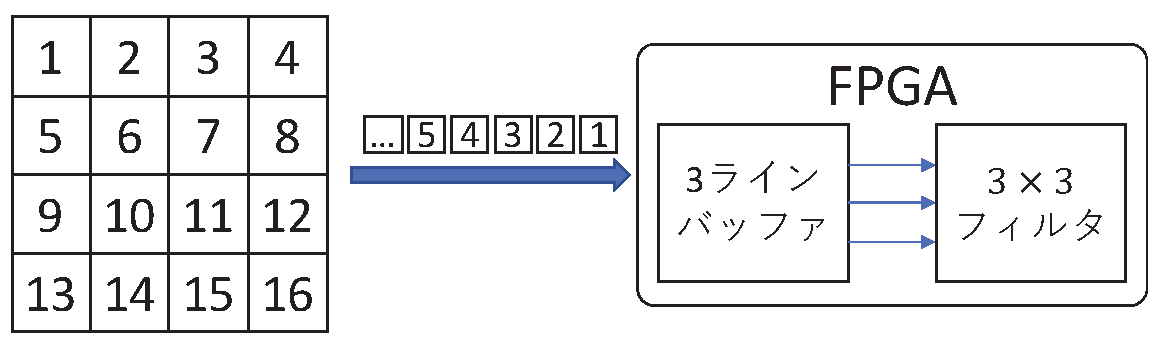
\includegraphics[width=0.7\linewidth]{../img/raster.pdf}
		\caption{システム構成}
		\label{img:raster}
	\end{figure}
\end{frame}

\section{3ラインバッファとは}
\begin{frame}
	\frametitle{3ラインバッファとは}
	\begin{itemize}
		\item
			$3\!\times\!3$のフィルタを計算に必要なピクセルの値を提供
		\item
			1列ずつ出てくる
	\end{itemize}
	\begin{figure}[ht]
		\centering
		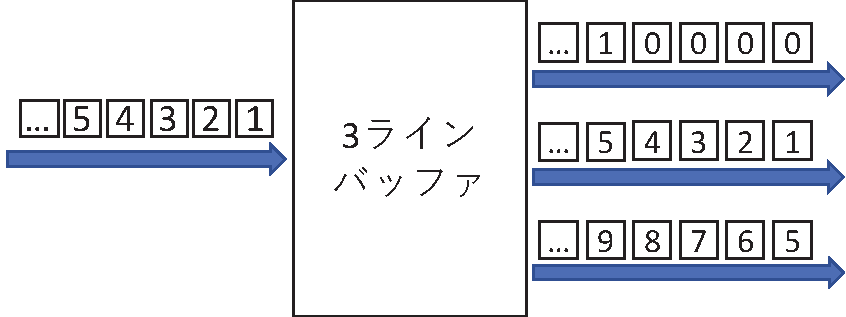
\includegraphics[width=0.5\linewidth]{../img/3lb.pdf}
		\caption{3ラインバッファの動作}
		\label{img:3linebuf}
	\end{figure}
	\vfill
	\begin{itemize}
		\item
			後段の回路では、この出力をレジスタに入れ、計算を行う
		\item
			計算をパイプライン化し、スループットを向上させること
	\end{itemize}
\end{frame}

\begin{frame}
	\frametitle{3ラインバッファの構成}
	\begin{itemize}
		\item
			FIFO IP Coreを3つ使って構成できる
	\end{itemize}
	\begin{figure}[ht]
		\centering
		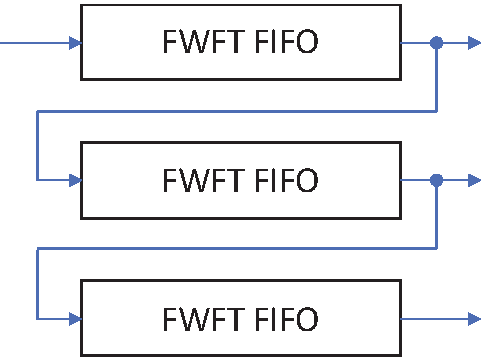
\includegraphics[width=0.4\linewidth]{../img/3lb_fifo.pdf}
		\caption{3ラインバッファの概念図}
		\label{img:3lb_fifo}
	\end{figure}
\end{frame}

\end{document}
